\documentclass{standalone}
\usepackage{tikz}
\usetikzlibrary{patterns, positioning}


\begin{document}
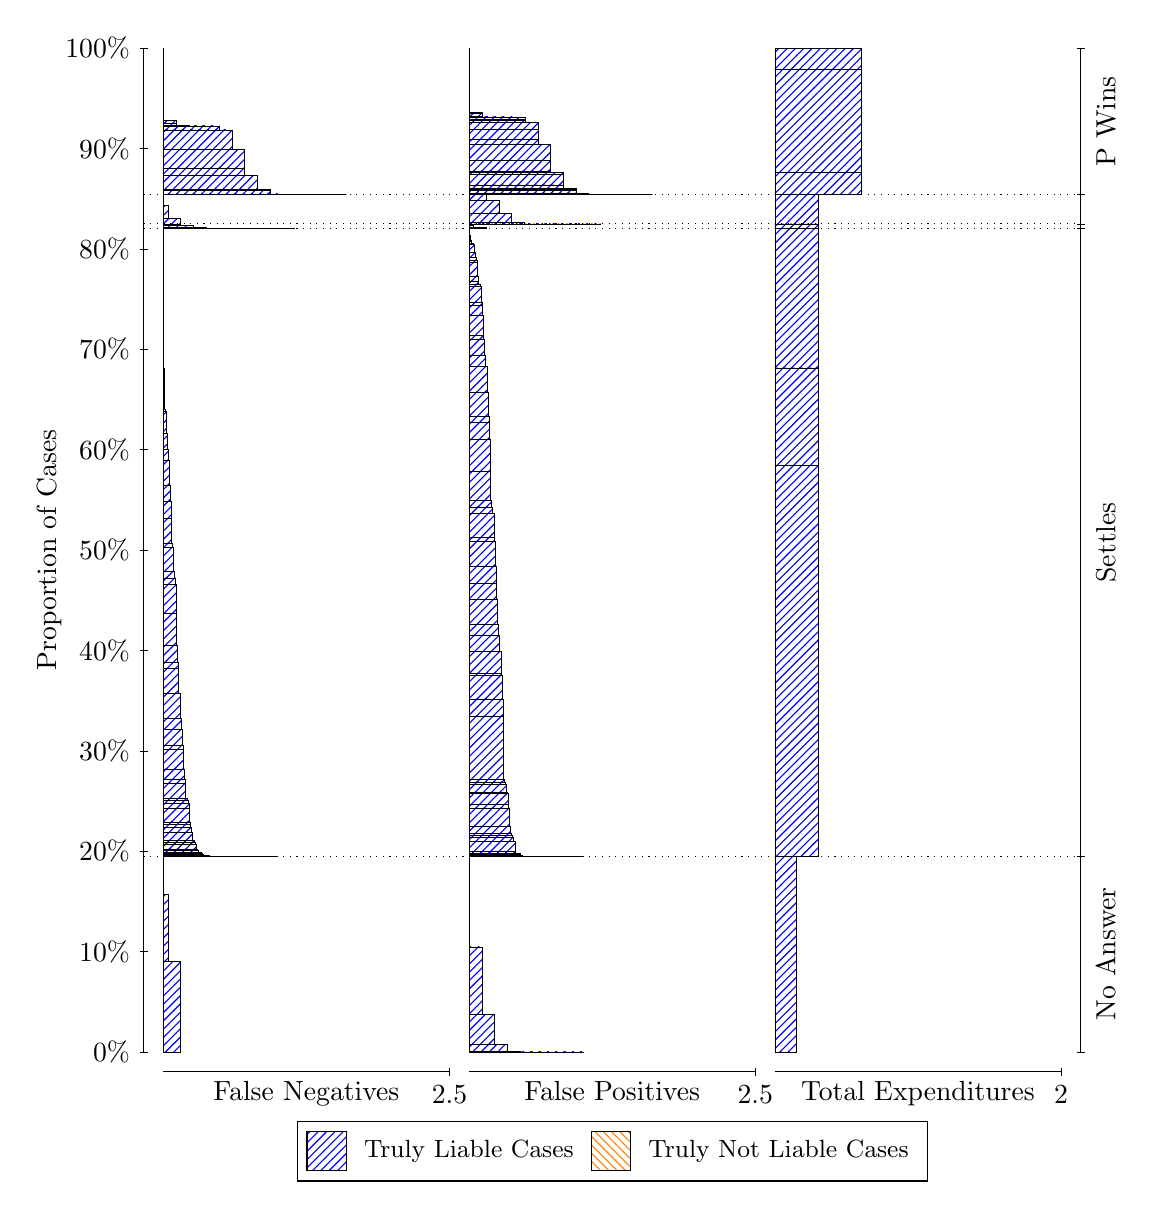
\begin{tikzpicture}
\draw[black, very thin] (1.5,1.75) -- (1.5,14.5);
\node[rotate=90, text=black, anchor=center] at (0.3, 8.125) {Proportion of Cases};
\draw[black, very thin] (1.45,1.75) -- (1.55,1.75);
\node[text=black, anchor=east] at (1.45, 1.75) {0\%};
\draw[black, very thin] (1.45,3.025) -- (1.55,3.025);
\node[text=black, anchor=east] at (1.45, 3.025) {10\%};
\draw[black, very thin] (1.45,4.3) -- (1.55,4.3);
\node[text=black, anchor=east] at (1.45, 4.3) {20\%};
\draw[black, very thin] (1.45,5.575) -- (1.55,5.575);
\node[text=black, anchor=east] at (1.45, 5.575) {30\%};
\draw[black, very thin] (1.45,6.85) -- (1.55,6.85);
\node[text=black, anchor=east] at (1.45, 6.85) {40\%};
\draw[black, very thin] (1.45,8.125) -- (1.55,8.125);
\node[text=black, anchor=east] at (1.45, 8.125) {50\%};
\draw[black, very thin] (1.45,9.4) -- (1.55,9.4);
\node[text=black, anchor=east] at (1.45, 9.4) {60\%};
\draw[black, very thin] (1.45,10.675) -- (1.55,10.675);
\node[text=black, anchor=east] at (1.45, 10.675) {70\%};
\draw[black, very thin] (1.45,11.95) -- (1.55,11.95);
\node[text=black, anchor=east] at (1.45, 11.95) {80\%};
\draw[black, very thin] (1.45,13.225) -- (1.55,13.225);
\node[text=black, anchor=east] at (1.45, 13.225) {90\%};
\draw[black, very thin] (1.45,14.5) -- (1.55,14.5);
\node[text=black, anchor=east] at (1.45, 14.5) {100\%};

\draw[black, very thin] (13.4,1.75) -- (13.4,14.5);
\draw[black, very thin] (13.35,1.75) -- (13.45,1.75);
\node[anchor=west] at (13.35, 1.75) {};
\draw[black, very thin] (13.35,4.2363) -- (13.45,4.2363);
\node[anchor=west] at (13.35, 4.2363) {};
\draw[black, very thin] (13.35,12.209) -- (13.45,12.209);
\node[anchor=west] at (13.35, 12.209) {};
\draw[black, very thin] (13.35,12.267) -- (13.45,12.267);
\node[anchor=west] at (13.35, 12.267) {};
\draw[black, very thin] (13.35,12.637) -- (13.45,12.637);
\node[anchor=west] at (13.35, 12.637) {};
\draw[black, very thin] (13.35,14.5) -- (13.45,14.5);
\node[anchor=west] at (13.35, 14.5) {};

\draw[black, very thin, pattern color=blue, pattern=north east lines] (1.75,1.75) rectangle (1.968,2.9018);
\draw[black, very thin, pattern color=blue, pattern=north east lines] (1.75,2.9018) rectangle (1.8065,3.7553);
\draw[black, very thin, pattern color=orange, pattern=north west lines] (1.75,3.7553) rectangle (1.75,3.7553);
\draw[black, very thin, pattern color=blue, pattern=north east lines] (1.75,3.7553) rectangle (1.75,4.2363);
\draw[black, very thin, pattern color=blue, pattern=north east lines] (1.75,4.2363) rectangle (3.2033,4.2363);
\draw[black, very thin, pattern color=blue, pattern=north east lines] (1.75,4.2363) rectangle (3.1307,4.2363);
\draw[black, very thin, pattern color=blue, pattern=north east lines] (1.75,4.2363) rectangle (3.058,4.2363);
\draw[black, very thin, pattern color=blue, pattern=north east lines] (1.75,4.2363) rectangle (3.0419,4.2363);
\draw[black, very thin, pattern color=blue, pattern=north east lines] (1.75,4.2363) rectangle (2.9853,4.2363);
\draw[black, very thin, pattern color=blue, pattern=north east lines] (1.75,4.2363) rectangle (2.9692,4.2363);
\draw[black, very thin, pattern color=blue, pattern=north east lines] (1.75,4.2363) rectangle (2.9127,4.2363);
\draw[black, very thin, pattern color=blue, pattern=north east lines] (1.75,4.2363) rectangle (2.8965,4.2363);
\draw[black, very thin, pattern color=blue, pattern=north east lines] (1.75,4.2363) rectangle (2.8804,4.2363);
\draw[black, very thin, pattern color=blue, pattern=north east lines] (1.75,4.2363) rectangle (2.84,4.2363);
\draw[black, very thin, pattern color=blue, pattern=north east lines] (1.75,4.2363) rectangle (2.8239,4.2363);
\draw[black, very thin, pattern color=blue, pattern=north east lines] (1.75,4.2363) rectangle (2.8077,4.2363);
\draw[black, very thin, pattern color=blue, pattern=north east lines] (1.75,4.2363) rectangle (2.7673,4.2363);
\draw[black, very thin, pattern color=blue, pattern=north east lines] (1.75,4.2363) rectangle (2.7512,4.2363);
\draw[black, very thin, pattern color=blue, pattern=north east lines] (1.75,4.2363) rectangle (2.735,4.2363);
\draw[black, very thin, pattern color=blue, pattern=north east lines] (1.75,4.2363) rectangle (2.7189,4.2363);
\draw[black, very thin, pattern color=blue, pattern=north east lines] (1.75,4.2363) rectangle (2.6947,4.2363);
\draw[black, very thin, pattern color=blue, pattern=north east lines] (1.75,4.2363) rectangle (2.6785,4.2363);
\draw[black, very thin, pattern color=blue, pattern=north east lines] (1.75,4.2363) rectangle (2.6624,4.2363);
\draw[black, very thin, pattern color=blue, pattern=north east lines] (1.75,4.2363) rectangle (2.6462,4.2363);
\draw[black, very thin, pattern color=blue, pattern=north east lines] (1.75,4.2363) rectangle (2.622,4.2363);
\draw[black, very thin, pattern color=blue, pattern=north east lines] (1.75,4.2363) rectangle (2.6059,4.2363);
\draw[black, very thin, pattern color=blue, pattern=north east lines] (1.75,4.2363) rectangle (2.5897,4.2363);
\draw[black, very thin, pattern color=blue, pattern=north east lines] (1.75,4.2363) rectangle (2.5736,4.2363);
\draw[black, very thin, pattern color=blue, pattern=north east lines] (1.75,4.2363) rectangle (2.5574,4.2363);
\draw[black, very thin, pattern color=blue, pattern=north east lines] (1.75,4.2363) rectangle (2.5493,4.2363);
\draw[black, very thin, pattern color=blue, pattern=north east lines] (1.75,4.2363) rectangle (2.5332,4.2363);
\draw[black, very thin, pattern color=blue, pattern=north east lines] (1.75,4.2363) rectangle (2.517,4.2363);
\draw[black, very thin, pattern color=blue, pattern=north east lines] (1.75,4.2363) rectangle (2.5009,4.2363);
\draw[black, very thin, pattern color=blue, pattern=north east lines] (1.75,4.2363) rectangle (2.4847,4.2363);
\draw[black, very thin, pattern color=blue, pattern=north east lines] (1.75,4.2363) rectangle (2.4767,4.2363);
\draw[black, very thin, pattern color=blue, pattern=north east lines] (1.75,4.2363) rectangle (2.4605,4.2363);
\draw[black, very thin, pattern color=blue, pattern=north east lines] (1.75,4.2363) rectangle (2.4444,4.2364);
\draw[black, very thin, pattern color=blue, pattern=north east lines] (1.75,4.2364) rectangle (2.4282,4.2364);
\draw[black, very thin, pattern color=blue, pattern=north east lines] (1.75,4.2364) rectangle (2.4121,4.2364);
\draw[black, very thin, pattern color=blue, pattern=north east lines] (1.75,4.2364) rectangle (2.404,4.237);
\draw[black, very thin, pattern color=blue, pattern=north east lines] (1.75,4.237) rectangle (2.3959,4.237);
\draw[black, very thin, pattern color=blue, pattern=north east lines] (1.75,4.237) rectangle (2.3879,4.2371);
\draw[black, very thin, pattern color=blue, pattern=north east lines] (1.75,4.2371) rectangle (2.3717,4.2371);
\draw[black, very thin, pattern color=blue, pattern=north east lines] (1.75,4.2371) rectangle (2.3556,4.2376);
\draw[black, very thin, pattern color=blue, pattern=north east lines] (1.75,4.2376) rectangle (2.3394,4.2377);
\draw[black, very thin, pattern color=blue, pattern=north east lines] (1.75,4.2377) rectangle (2.3313,4.2429);
\draw[black, very thin, pattern color=blue, pattern=north east lines] (1.75,4.2429) rectangle (2.3233,4.2429);
\draw[black, very thin, pattern color=blue, pattern=north east lines] (1.75,4.2429) rectangle (2.3152,4.2436);
\draw[black, very thin, pattern color=blue, pattern=north east lines] (1.75,4.2436) rectangle (2.299,4.2442);
\draw[black, very thin, pattern color=blue, pattern=north east lines] (1.75,4.2442) rectangle (2.2829,4.2494);
\draw[black, very thin, pattern color=blue, pattern=north east lines] (1.75,4.2494) rectangle (2.2667,4.2521);
\draw[black, very thin, pattern color=blue, pattern=north east lines] (1.75,4.2521) rectangle (2.2587,4.2561);
\draw[black, very thin, pattern color=blue, pattern=north east lines] (1.75,4.2561) rectangle (2.2506,4.2569);
\draw[black, very thin, pattern color=blue, pattern=north east lines] (1.75,4.2569) rectangle (2.2425,4.2744);
\draw[black, very thin, pattern color=blue, pattern=north east lines] (1.75,4.2744) rectangle (2.2344,4.2771);
\draw[black, very thin, pattern color=blue, pattern=north east lines] (1.75,4.2771) rectangle (2.2264,4.2805);
\draw[black, very thin, pattern color=blue, pattern=north east lines] (1.75,4.2805) rectangle (2.2102,4.2824);
\draw[black, very thin, pattern color=blue, pattern=north east lines] (1.75,4.2824) rectangle (2.1941,4.3059);
\draw[black, very thin, pattern color=blue, pattern=north east lines] (1.75,4.3059) rectangle (2.186,4.3184);
\draw[black, very thin, pattern color=blue, pattern=north east lines] (1.75,4.3184) rectangle (2.1779,4.328);
\draw[black, very thin, pattern color=blue, pattern=north east lines] (1.75,4.328) rectangle (2.1699,4.3911);
\draw[black, very thin, pattern color=blue, pattern=north east lines] (1.75,4.3911) rectangle (2.1618,4.3941);
\draw[black, very thin, pattern color=blue, pattern=north east lines] (1.75,4.3941) rectangle (2.1537,4.4192);
\draw[black, very thin, pattern color=blue, pattern=north east lines] (1.75,4.4192) rectangle (2.1376,4.4418);
\draw[black, very thin, pattern color=blue, pattern=north east lines] (1.75,4.4418) rectangle (2.1214,4.538);
\draw[black, very thin, pattern color=blue, pattern=north east lines] (1.75,4.538) rectangle (2.1053,4.6049);
\draw[black, very thin, pattern color=blue, pattern=north east lines] (1.75,4.6049) rectangle (2.0972,4.6396);
\draw[black, very thin, pattern color=blue, pattern=north east lines] (1.75,4.6396) rectangle (2.0891,4.671);
\draw[black, very thin, pattern color=blue, pattern=north east lines] (1.75,4.671) rectangle (2.081,4.8393);
\draw[black, very thin, pattern color=blue, pattern=north east lines] (1.75,4.8393) rectangle (2.073,4.9024);
\draw[black, very thin, pattern color=blue, pattern=north east lines] (1.75,4.9024) rectangle (2.0649,4.9421);
\draw[black, very thin, pattern color=blue, pattern=north east lines] (1.75,4.9421) rectangle (2.0487,4.9738);
\draw[black, very thin, pattern color=blue, pattern=north east lines] (1.75,4.9738) rectangle (2.0326,5.1682);
\draw[black, very thin, pattern color=blue, pattern=north east lines] (1.75,5.1682) rectangle (2.0245,5.2166);
\draw[black, very thin, pattern color=blue, pattern=north east lines] (1.75,5.2166) rectangle (2.0164,5.3442);
\draw[black, very thin, pattern color=blue, pattern=north east lines] (1.75,5.3442) rectangle (2.0084,5.5908);
\draw[black, very thin, pattern color=blue, pattern=north east lines] (1.75,5.5908) rectangle (2.0003,5.6457);
\draw[black, very thin, pattern color=blue, pattern=north east lines] (1.75,5.6457) rectangle (1.9922,5.8478);
\draw[black, very thin, pattern color=blue, pattern=north east lines] (1.75,5.8478) rectangle (1.9761,5.987);
\draw[black, very thin, pattern color=blue, pattern=north east lines] (1.75,5.987) rectangle (1.9599,6.3112);
\draw[black, very thin, pattern color=blue, pattern=north east lines] (1.75,6.3112) rectangle (1.9438,6.6219);
\draw[black, very thin, pattern color=blue, pattern=north east lines] (1.75,6.6219) rectangle (1.9357,6.6987);
\draw[black, very thin, pattern color=blue, pattern=north east lines] (1.75,6.6987) rectangle (1.9276,6.9177);
\draw[black, very thin, pattern color=blue, pattern=north east lines] (1.75,6.9177) rectangle (1.9196,7.318);
\draw[black, very thin, pattern color=blue, pattern=north east lines] (1.75,7.318) rectangle (1.9115,7.6855);
\draw[black, very thin, pattern color=blue, pattern=north east lines] (1.75,7.6855) rectangle (1.9034,7.7716);
\draw[black, very thin, pattern color=blue, pattern=north east lines] (1.75,7.7716) rectangle (1.8873,7.8511);
\draw[black, very thin, pattern color=blue, pattern=north east lines] (1.75,7.8511) rectangle (1.8711,8.1613);
\draw[black, very thin, pattern color=blue, pattern=north east lines] (1.75,8.1613) rectangle (1.863,8.2154);
\draw[black, very thin, pattern color=blue, pattern=north east lines] (1.75,8.2154) rectangle (1.855,8.5227);
\draw[black, very thin, pattern color=blue, pattern=north east lines] (1.75,8.5227) rectangle (1.8469,8.7444);
\draw[black, very thin, pattern color=blue, pattern=north east lines] (1.75,8.7444) rectangle (1.8388,8.9482);
\draw[black, very thin, pattern color=blue, pattern=north east lines] (1.75,8.9482) rectangle (1.8307,9.2626);
\draw[black, very thin, pattern color=blue, pattern=north east lines] (1.75,9.2626) rectangle (1.8146,9.4005);
\draw[black, very thin, pattern color=blue, pattern=north east lines] (1.75,9.4005) rectangle (1.7984,9.6123);
\draw[black, very thin, pattern color=blue, pattern=north east lines] (1.75,9.6123) rectangle (1.7823,9.8812);
\draw[black, very thin, pattern color=blue, pattern=north east lines] (1.75,9.8812) rectangle (1.7742,9.9115);
\draw[black, very thin, pattern color=blue, pattern=north east lines] (1.75,9.9115) rectangle (1.7661,10.211);
\draw[black, very thin, pattern color=blue, pattern=north east lines] (1.75,10.211) rectangle (1.7581,10.428);
\draw[black, very thin, pattern color=orange, pattern=north west lines] (1.75,10.428) rectangle (1.75,10.428);
\draw[black, very thin, pattern color=blue, pattern=north east lines] (1.75,10.428) rectangle (1.75,12.209);
\draw[black, very thin, pattern color=blue, pattern=north east lines] (1.75,12.209) rectangle (3.4213,12.209);
\draw[black, very thin, pattern color=blue, pattern=north east lines] (1.75,12.209) rectangle (3.2599,12.209);
\draw[black, very thin, pattern color=blue, pattern=north east lines] (1.75,12.209) rectangle (3.0984,12.209);
\draw[black, very thin, pattern color=blue, pattern=north east lines] (1.75,12.209) rectangle (2.9369,12.209);
\draw[black, very thin, pattern color=blue, pattern=north east lines] (1.75,12.209) rectangle (2.7754,12.209);
\draw[black, very thin, pattern color=blue, pattern=north east lines] (1.75,12.209) rectangle (2.6139,12.209);
\draw[black, very thin, pattern color=blue, pattern=north east lines] (1.75,12.209) rectangle (2.4524,12.21);
\draw[black, very thin, pattern color=blue, pattern=north east lines] (1.75,12.21) rectangle (2.291,12.225);
\draw[black, very thin, pattern color=blue, pattern=north east lines] (1.75,12.225) rectangle (2.1295,12.252);
\draw[black, very thin, pattern color=blue, pattern=north east lines] (1.75,12.252) rectangle (1.968,12.267);
\draw[black, very thin, pattern color=orange, pattern=north west lines] (1.75,12.267) rectangle (1.75,12.267);
\draw[black, very thin, pattern color=blue, pattern=north east lines] (1.75,12.267) rectangle (1.968,12.341);
\draw[black, very thin, pattern color=blue, pattern=north east lines] (1.75,12.341) rectangle (1.8065,12.5);
\draw[black, very thin, pattern color=orange, pattern=north west lines] (1.75,12.5) rectangle (1.75,12.5);
\draw[black, very thin, pattern color=blue, pattern=north east lines] (1.75,12.5) rectangle (1.75,12.637);
\draw[black, very thin, pattern color=blue, pattern=north east lines] (1.75,12.637) rectangle (4.0753,12.637);
\draw[black, very thin, pattern color=blue, pattern=north east lines] (1.75,12.637) rectangle (3.9139,12.637);
\draw[black, very thin, pattern color=blue, pattern=north east lines] (1.75,12.637) rectangle (3.7524,12.637);
\draw[black, very thin, pattern color=blue, pattern=north east lines] (1.75,12.637) rectangle (3.5909,12.638);
\draw[black, very thin, pattern color=blue, pattern=north east lines] (1.75,12.638) rectangle (3.4294,12.639);
\draw[black, very thin, pattern color=blue, pattern=north east lines] (1.75,12.639) rectangle (3.2679,12.643);
\draw[black, very thin, pattern color=blue, pattern=north east lines] (1.75,12.643) rectangle (3.2679,12.649);
\draw[black, very thin, pattern color=blue, pattern=north east lines] (1.75,12.649) rectangle (3.1064,12.699);
\draw[black, very thin, pattern color=blue, pattern=north east lines] (1.75,12.699) rectangle (3.1064,12.704);
\draw[black, very thin, pattern color=blue, pattern=north east lines] (1.75,12.704) rectangle (2.945,12.884);
\draw[black, very thin, pattern color=blue, pattern=north east lines] (1.75,12.884) rectangle (2.8804,12.884);
\draw[black, very thin, pattern color=blue, pattern=north east lines] (1.75,12.884) rectangle (2.7835,12.979);
\draw[black, very thin, pattern color=blue, pattern=north east lines] (1.75,12.979) rectangle (2.7835,13.214);
\draw[black, very thin, pattern color=blue, pattern=north east lines] (1.75,13.214) rectangle (2.7189,13.214);
\draw[black, very thin, pattern color=blue, pattern=north east lines] (1.75,13.214) rectangle (2.7189,13.214);
\draw[black, very thin, pattern color=blue, pattern=north east lines] (1.75,13.214) rectangle (2.622,13.459);
\draw[black, very thin, pattern color=blue, pattern=north east lines] (1.75,13.459) rectangle (2.5574,13.459);
\draw[black, very thin, pattern color=blue, pattern=north east lines] (1.75,13.459) rectangle (2.4605,13.46);
\draw[black, very thin, pattern color=blue, pattern=north east lines] (1.75,13.46) rectangle (2.4605,13.51);
\draw[black, very thin, pattern color=blue, pattern=north east lines] (1.75,13.51) rectangle (2.4605,13.511);
\draw[black, very thin, pattern color=blue, pattern=north east lines] (1.75,13.511) rectangle (2.3959,13.511);
\draw[black, very thin, pattern color=blue, pattern=north east lines] (1.75,13.511) rectangle (2.3959,13.511);
\draw[black, very thin, pattern color=blue, pattern=north east lines] (1.75,13.511) rectangle (2.299,13.512);
\draw[black, very thin, pattern color=blue, pattern=north east lines] (1.75,13.512) rectangle (2.299,13.512);
\draw[black, very thin, pattern color=blue, pattern=north east lines] (1.75,13.512) rectangle (2.2344,13.512);
\draw[black, very thin, pattern color=blue, pattern=north east lines] (1.75,13.512) rectangle (2.2344,13.512);
\draw[black, very thin, pattern color=blue, pattern=north east lines] (1.75,13.512) rectangle (2.2344,13.512);
\draw[black, very thin, pattern color=blue, pattern=north east lines] (1.75,13.512) rectangle (2.1376,13.512);
\draw[black, very thin, pattern color=blue, pattern=north east lines] (1.75,13.512) rectangle (2.1376,13.512);
\draw[black, very thin, pattern color=blue, pattern=north east lines] (1.75,13.512) rectangle (2.073,13.512);
\draw[black, very thin, pattern color=blue, pattern=north east lines] (1.75,13.512) rectangle (2.073,13.516);
\draw[black, very thin, pattern color=blue, pattern=north east lines] (1.75,13.516) rectangle (1.9761,13.516);
\draw[black, very thin, pattern color=blue, pattern=north east lines] (1.75,13.516) rectangle (1.9761,13.516);
\draw[black, very thin, pattern color=blue, pattern=north east lines] (1.75,13.516) rectangle (1.9115,13.541);
\draw[black, very thin, pattern color=blue, pattern=north east lines] (1.75,13.541) rectangle (1.9115,13.55);
\draw[black, very thin, pattern color=blue, pattern=north east lines] (1.75,13.55) rectangle (1.9115,13.584);
\draw[black, very thin, pattern color=blue, pattern=north east lines] (1.75,13.584) rectangle (1.8146,13.584);
\draw[black, very thin, pattern color=blue, pattern=north east lines] (1.75,13.584) rectangle (1.8146,13.584);
\draw[black, very thin, pattern color=orange, pattern=north west lines] (1.75,13.584) rectangle (1.75,13.584);
\draw[black, very thin, pattern color=blue, pattern=north east lines] (1.75,13.584) rectangle (1.75,14.5);
\draw[black, very thin, pattern color=orange, pattern=north west lines] (5.6333,1.75) rectangle (7.0867,1.75);
\draw[black, very thin, pattern color=blue, pattern=north east lines] (5.6333,1.75) rectangle (7.0867,1.75);
\draw[black, very thin, pattern color=blue, pattern=north east lines] (5.6333,1.75) rectangle (6.9252,1.75);
\draw[black, very thin, pattern color=blue, pattern=north east lines] (5.6333,1.75) rectangle (6.7637,1.75);
\draw[black, very thin, pattern color=blue, pattern=north east lines] (5.6333,1.75) rectangle (6.6022,1.75);
\draw[black, very thin, pattern color=blue, pattern=north east lines] (5.6333,1.75) rectangle (6.4407,1.7503);
\draw[black, very thin, pattern color=blue, pattern=north east lines] (5.6333,1.7503) rectangle (6.2793,1.7582);
\draw[black, very thin, pattern color=blue, pattern=north east lines] (5.6333,1.7582) rectangle (6.1178,1.8431);
\draw[black, very thin, pattern color=blue, pattern=north east lines] (5.6333,1.8431) rectangle (5.9563,2.231);
\draw[black, very thin, pattern color=blue, pattern=north east lines] (5.6333,2.231) rectangle (5.7948,3.0845);
\draw[black, very thin, pattern color=blue, pattern=north east lines] (5.6333,3.0845) rectangle (5.6333,4.2363);
\draw[black, very thin, pattern color=orange, pattern=north west lines] (5.6333,4.2363) rectangle (7.0867,4.2363);
\draw[black, very thin, pattern color=blue, pattern=north east lines] (5.6333,4.2363) rectangle (7.0867,4.2363);
\draw[black, very thin, pattern color=orange, pattern=north west lines] (5.6333,4.2363) rectangle (7.014,4.2363);
\draw[black, very thin, pattern color=blue, pattern=north east lines] (5.6333,4.2363) rectangle (7.014,4.2363);
\draw[black, very thin, pattern color=orange, pattern=north west lines] (5.6333,4.2363) rectangle (6.9413,4.2363);
\draw[black, very thin, pattern color=blue, pattern=north east lines] (5.6333,4.2363) rectangle (6.9413,4.2363);
\draw[black, very thin, pattern color=blue, pattern=north east lines] (5.6333,4.2363) rectangle (6.9252,4.2363);
\draw[black, very thin, pattern color=orange, pattern=north west lines] (5.6333,4.2363) rectangle (6.8687,4.2363);
\draw[black, very thin, pattern color=blue, pattern=north east lines] (5.6333,4.2363) rectangle (6.8687,4.2363);
\draw[black, very thin, pattern color=blue, pattern=north east lines] (5.6333,4.2363) rectangle (6.8525,4.2363);
\draw[black, very thin, pattern color=orange, pattern=north west lines] (5.6333,4.2363) rectangle (6.796,4.2363);
\draw[black, very thin, pattern color=blue, pattern=north east lines] (5.6333,4.2363) rectangle (6.796,4.2363);
\draw[black, very thin, pattern color=blue, pattern=north east lines] (5.6333,4.2363) rectangle (6.7799,4.2363);
\draw[black, very thin, pattern color=blue, pattern=north east lines] (5.6333,4.2363) rectangle (6.7637,4.2363);
\draw[black, very thin, pattern color=orange, pattern=north west lines] (5.6333,4.2363) rectangle (6.7233,4.2363);
\draw[black, very thin, pattern color=blue, pattern=north east lines] (5.6333,4.2363) rectangle (6.7233,4.2363);
\draw[black, very thin, pattern color=blue, pattern=north east lines] (5.6333,4.2363) rectangle (6.7072,4.2363);
\draw[black, very thin, pattern color=blue, pattern=north east lines] (5.6333,4.2363) rectangle (6.691,4.2363);
\draw[black, very thin, pattern color=orange, pattern=north west lines] (5.6333,4.2363) rectangle (6.6507,4.2363);
\draw[black, very thin, pattern color=blue, pattern=north east lines] (5.6333,4.2363) rectangle (6.6507,4.2363);
\draw[black, very thin, pattern color=blue, pattern=north east lines] (5.6333,4.2363) rectangle (6.6345,4.2363);
\draw[black, very thin, pattern color=blue, pattern=north east lines] (5.6333,4.2363) rectangle (6.6184,4.2363);
\draw[black, very thin, pattern color=blue, pattern=north east lines] (5.6333,4.2363) rectangle (6.6022,4.2363);
\draw[black, very thin, pattern color=orange, pattern=north west lines] (5.6333,4.2363) rectangle (6.578,4.2363);
\draw[black, very thin, pattern color=blue, pattern=north east lines] (5.6333,4.2363) rectangle (6.578,4.2363);
\draw[black, very thin, pattern color=blue, pattern=north east lines] (5.6333,4.2363) rectangle (6.5619,4.2363);
\draw[black, very thin, pattern color=blue, pattern=north east lines] (5.6333,4.2363) rectangle (6.5457,4.2363);
\draw[black, very thin, pattern color=blue, pattern=north east lines] (5.6333,4.2363) rectangle (6.5296,4.2363);
\draw[black, very thin, pattern color=orange, pattern=north west lines] (5.6333,4.2363) rectangle (6.5053,4.2363);
\draw[black, very thin, pattern color=blue, pattern=north east lines] (5.6333,4.2363) rectangle (6.5053,4.2363);
\draw[black, very thin, pattern color=blue, pattern=north east lines] (5.6333,4.2363) rectangle (6.4892,4.2363);
\draw[black, very thin, pattern color=blue, pattern=north east lines] (5.6333,4.2363) rectangle (6.473,4.2364);
\draw[black, very thin, pattern color=blue, pattern=north east lines] (5.6333,4.2364) rectangle (6.4569,4.2364);
\draw[black, very thin, pattern color=blue, pattern=north east lines] (5.6333,4.2364) rectangle (6.4407,4.2364);
\draw[black, very thin, pattern color=orange, pattern=north west lines] (5.6333,4.2364) rectangle (6.4327,4.2364);
\draw[black, very thin, pattern color=blue, pattern=north east lines] (5.6333,4.2364) rectangle (6.4327,4.2365);
\draw[black, very thin, pattern color=blue, pattern=north east lines] (5.6333,4.2365) rectangle (6.4165,4.2365);
\draw[black, very thin, pattern color=blue, pattern=north east lines] (5.6333,4.2365) rectangle (6.4004,4.2365);
\draw[black, very thin, pattern color=blue, pattern=north east lines] (5.6333,4.2365) rectangle (6.3842,4.237);
\draw[black, very thin, pattern color=blue, pattern=north east lines] (5.6333,4.237) rectangle (6.3681,4.2371);
\draw[black, very thin, pattern color=orange, pattern=north west lines] (5.6333,4.2371) rectangle (6.36,4.2371);
\draw[black, very thin, pattern color=blue, pattern=north east lines] (5.6333,4.2371) rectangle (6.36,4.239);
\draw[black, very thin, pattern color=blue, pattern=north east lines] (5.6333,4.239) rectangle (6.3439,4.2397);
\draw[black, very thin, pattern color=blue, pattern=north east lines] (5.6333,4.2397) rectangle (6.3277,4.2402);
\draw[black, very thin, pattern color=blue, pattern=north east lines] (5.6333,4.2402) rectangle (6.3116,4.2454);
\draw[black, very thin, pattern color=blue, pattern=north east lines] (5.6333,4.2454) rectangle (6.2954,4.247);
\draw[black, very thin, pattern color=orange, pattern=north west lines] (5.6333,4.247) rectangle (6.2873,4.247);
\draw[black, very thin, pattern color=blue, pattern=north east lines] (5.6333,4.247) rectangle (6.2873,4.2671);
\draw[black, very thin, pattern color=blue, pattern=north east lines] (5.6333,4.2671) rectangle (6.2793,4.2677);
\draw[black, very thin, pattern color=blue, pattern=north east lines] (5.6333,4.2677) rectangle (6.2712,4.2738);
\draw[black, very thin, pattern color=blue, pattern=north east lines] (5.6333,4.2738) rectangle (6.255,4.2758);
\draw[black, very thin, pattern color=blue, pattern=north east lines] (5.6333,4.2758) rectangle (6.2389,4.2777);
\draw[black, very thin, pattern color=blue, pattern=north east lines] (5.6333,4.2777) rectangle (6.2227,4.3022);
\draw[black, very thin, pattern color=orange, pattern=north west lines] (5.6333,4.3022) rectangle (6.2147,4.3022);
\draw[black, very thin, pattern color=blue, pattern=north east lines] (5.6333,4.3022) rectangle (6.2147,4.4259);
\draw[black, very thin, pattern color=blue, pattern=north east lines] (5.6333,4.4259) rectangle (6.2066,4.4278);
\draw[black, very thin, pattern color=blue, pattern=north east lines] (5.6333,4.4278) rectangle (6.1985,4.4728);
\draw[black, very thin, pattern color=blue, pattern=north east lines] (5.6333,4.4728) rectangle (6.1824,4.4995);
\draw[black, very thin, pattern color=blue, pattern=north east lines] (5.6333,4.4995) rectangle (6.1662,4.5212);
\draw[black, very thin, pattern color=blue, pattern=north east lines] (5.6333,4.5212) rectangle (6.1501,4.6159);
\draw[black, very thin, pattern color=orange, pattern=north west lines] (5.6333,4.6159) rectangle (6.142,4.6159);
\draw[black, very thin, pattern color=blue, pattern=north east lines] (5.6333,4.6159) rectangle (6.142,4.8502);
\draw[black, very thin, pattern color=blue, pattern=north east lines] (5.6333,4.8502) rectangle (6.1339,4.8914);
\draw[black, very thin, pattern color=blue, pattern=north east lines] (5.6333,4.8914) rectangle (6.1259,5.0379);
\draw[black, very thin, pattern color=blue, pattern=north east lines] (5.6333,5.0379) rectangle (6.1178,5.0508);
\draw[black, very thin, pattern color=blue, pattern=north east lines] (5.6333,5.0508) rectangle (6.1097,5.1475);
\draw[black, very thin, pattern color=blue, pattern=north east lines] (5.6333,5.1475) rectangle (6.0936,5.179);
\draw[black, very thin, pattern color=blue, pattern=north east lines] (5.6333,5.179) rectangle (6.0774,5.2109);
\draw[black, very thin, pattern color=orange, pattern=north west lines] (5.6333,5.2109) rectangle (6.0693,5.2109);
\draw[black, very thin, pattern color=blue, pattern=north east lines] (5.6333,5.2109) rectangle (6.0693,6.0171);
\draw[black, very thin, pattern color=blue, pattern=north east lines] (5.6333,6.0171) rectangle (6.0613,6.2335);
\draw[black, very thin, pattern color=blue, pattern=north east lines] (5.6333,6.2335) rectangle (6.0532,6.5335);
\draw[black, very thin, pattern color=blue, pattern=north east lines] (5.6333,6.5335) rectangle (6.0451,6.5637);
\draw[black, very thin, pattern color=blue, pattern=north east lines] (5.6333,6.5637) rectangle (6.037,6.8327);
\draw[black, very thin, pattern color=blue, pattern=north east lines] (5.6333,6.8327) rectangle (6.0209,7.0445);
\draw[black, very thin, pattern color=blue, pattern=north east lines] (5.6333,7.0445) rectangle (6.0047,7.1823);
\draw[black, very thin, pattern color=blue, pattern=north east lines] (5.6333,7.1823) rectangle (5.9886,7.4967);
\draw[black, very thin, pattern color=blue, pattern=north east lines] (5.6333,7.4967) rectangle (5.9805,7.7005);
\draw[black, very thin, pattern color=blue, pattern=north east lines] (5.6333,7.7005) rectangle (5.9724,7.9222);
\draw[black, very thin, pattern color=blue, pattern=north east lines] (5.6333,7.9222) rectangle (5.9644,8.2295);
\draw[black, very thin, pattern color=blue, pattern=north east lines] (5.6333,8.2295) rectangle (5.9563,8.2836);
\draw[black, very thin, pattern color=blue, pattern=north east lines] (5.6333,8.2836) rectangle (5.9482,8.5939);
\draw[black, very thin, pattern color=blue, pattern=north east lines] (5.6333,8.5939) rectangle (5.9321,8.6733);
\draw[black, very thin, pattern color=blue, pattern=north east lines] (5.6333,8.6733) rectangle (5.9159,8.7594);
\draw[black, very thin, pattern color=blue, pattern=north east lines] (5.6333,8.7594) rectangle (5.9079,9.1269);
\draw[black, very thin, pattern color=blue, pattern=north east lines] (5.6333,9.1269) rectangle (5.8998,9.5272);
\draw[black, very thin, pattern color=blue, pattern=north east lines] (5.6333,9.5272) rectangle (5.8917,9.7462);
\draw[black, very thin, pattern color=blue, pattern=north east lines] (5.6333,9.7462) rectangle (5.8836,9.823);
\draw[black, very thin, pattern color=blue, pattern=north east lines] (5.6333,9.823) rectangle (5.8756,10.134);
\draw[black, very thin, pattern color=blue, pattern=north east lines] (5.6333,10.134) rectangle (5.8594,10.458);
\draw[black, very thin, pattern color=blue, pattern=north east lines] (5.6333,10.458) rectangle (5.8433,10.597);
\draw[black, very thin, pattern color=blue, pattern=north east lines] (5.6333,10.597) rectangle (5.8271,10.799);
\draw[black, very thin, pattern color=blue, pattern=north east lines] (5.6333,10.799) rectangle (5.819,10.854);
\draw[black, very thin, pattern color=blue, pattern=north east lines] (5.6333,10.854) rectangle (5.811,11.101);
\draw[black, very thin, pattern color=blue, pattern=north east lines] (5.6333,11.101) rectangle (5.8029,11.228);
\draw[black, very thin, pattern color=blue, pattern=north east lines] (5.6333,11.228) rectangle (5.7948,11.277);
\draw[black, very thin, pattern color=blue, pattern=north east lines] (5.6333,11.277) rectangle (5.7867,11.471);
\draw[black, very thin, pattern color=blue, pattern=north east lines] (5.6333,11.471) rectangle (5.7706,11.503);
\draw[black, very thin, pattern color=blue, pattern=north east lines] (5.6333,11.503) rectangle (5.7544,11.543);
\draw[black, very thin, pattern color=blue, pattern=north east lines] (5.6333,11.543) rectangle (5.7464,11.606);
\draw[black, very thin, pattern color=blue, pattern=north east lines] (5.6333,11.606) rectangle (5.7383,11.774);
\draw[black, very thin, pattern color=blue, pattern=north east lines] (5.6333,11.774) rectangle (5.7302,11.805);
\draw[black, very thin, pattern color=blue, pattern=north east lines] (5.6333,11.805) rectangle (5.7221,11.84);
\draw[black, very thin, pattern color=blue, pattern=north east lines] (5.6333,11.84) rectangle (5.7141,11.907);
\draw[black, very thin, pattern color=blue, pattern=north east lines] (5.6333,11.907) rectangle (5.6979,12.003);
\draw[black, very thin, pattern color=blue, pattern=north east lines] (5.6333,12.003) rectangle (5.6818,12.026);
\draw[black, very thin, pattern color=blue, pattern=north east lines] (5.6333,12.026) rectangle (5.6656,12.051);
\draw[black, very thin, pattern color=blue, pattern=north east lines] (5.6333,12.051) rectangle (5.6576,12.054);
\draw[black, very thin, pattern color=blue, pattern=north east lines] (5.6333,12.054) rectangle (5.6495,12.117);
\draw[black, very thin, pattern color=blue, pattern=north east lines] (5.6333,12.117) rectangle (5.6414,12.127);
\draw[black, very thin, pattern color=blue, pattern=north east lines] (5.6333,12.127) rectangle (5.6333,12.209);
\draw[black, very thin, pattern color=orange, pattern=north west lines] (5.6333,12.209) rectangle (5.8513,12.209);
\draw[black, very thin, pattern color=blue, pattern=north east lines] (5.6333,12.209) rectangle (5.8513,12.223);
\draw[black, very thin, pattern color=blue, pattern=north east lines] (5.6333,12.223) rectangle (5.6899,12.25);
\draw[black, very thin, pattern color=blue, pattern=north east lines] (5.6333,12.25) rectangle (5.6333,12.267);
\draw[black, very thin, pattern color=orange, pattern=north west lines] (5.6333,12.267) rectangle (7.3047,12.267);
\draw[black, very thin, pattern color=blue, pattern=north east lines] (5.6333,12.267) rectangle (7.3047,12.267);
\draw[black, very thin, pattern color=blue, pattern=north east lines] (5.6333,12.267) rectangle (7.1432,12.267);
\draw[black, very thin, pattern color=blue, pattern=north east lines] (5.6333,12.267) rectangle (6.9817,12.267);
\draw[black, very thin, pattern color=blue, pattern=north east lines] (5.6333,12.267) rectangle (6.8202,12.267);
\draw[black, very thin, pattern color=blue, pattern=north east lines] (5.6333,12.267) rectangle (6.6587,12.267);
\draw[black, very thin, pattern color=blue, pattern=north east lines] (5.6333,12.267) rectangle (6.4973,12.268);
\draw[black, very thin, pattern color=blue, pattern=north east lines] (5.6333,12.268) rectangle (6.3358,12.288);
\draw[black, very thin, pattern color=blue, pattern=north east lines] (5.6333,12.288) rectangle (6.1743,12.404);
\draw[black, very thin, pattern color=blue, pattern=north east lines] (5.6333,12.404) rectangle (6.0128,12.564);
\draw[black, very thin, pattern color=blue, pattern=north east lines] (5.6333,12.564) rectangle (5.8513,12.637);
\draw[black, very thin, pattern color=orange, pattern=north west lines] (5.6333,12.637) rectangle (7.9587,12.637);
\draw[black, very thin, pattern color=blue, pattern=north east lines] (5.6333,12.637) rectangle (7.9587,12.637);
\draw[black, very thin, pattern color=orange, pattern=north west lines] (5.6333,12.637) rectangle (7.7972,12.637);
\draw[black, very thin, pattern color=blue, pattern=north east lines] (5.6333,12.637) rectangle (7.7972,12.637);
\draw[black, very thin, pattern color=orange, pattern=north west lines] (5.6333,12.637) rectangle (7.6357,12.637);
\draw[black, very thin, pattern color=blue, pattern=north east lines] (5.6333,12.637) rectangle (7.6357,12.637);
\draw[black, very thin, pattern color=blue, pattern=north east lines] (5.6333,12.637) rectangle (7.4742,12.638);
\draw[black, very thin, pattern color=orange, pattern=north west lines] (5.6333,12.638) rectangle (7.4742,12.638);
\draw[black, very thin, pattern color=blue, pattern=north east lines] (5.6333,12.638) rectangle (7.4742,12.638);
\draw[black, very thin, pattern color=blue, pattern=north east lines] (5.6333,12.638) rectangle (7.3127,12.638);
\draw[black, very thin, pattern color=orange, pattern=north west lines] (5.6333,12.638) rectangle (7.3127,12.638);
\draw[black, very thin, pattern color=blue, pattern=north east lines] (5.6333,12.638) rectangle (7.3127,12.639);
\draw[black, very thin, pattern color=blue, pattern=north east lines] (5.6333,12.639) rectangle (7.1513,12.646);
\draw[black, very thin, pattern color=orange, pattern=north west lines] (5.6333,12.646) rectangle (7.1513,12.646);
\draw[black, very thin, pattern color=blue, pattern=north east lines] (5.6333,12.646) rectangle (7.1513,12.651);
\draw[black, very thin, pattern color=blue, pattern=north east lines] (5.6333,12.651) rectangle (6.9898,12.66);
\draw[black, very thin, pattern color=orange, pattern=north west lines] (5.6333,12.66) rectangle (6.9898,12.66);
\draw[black, very thin, pattern color=blue, pattern=north east lines] (5.6333,12.66) rectangle (6.9898,12.696);
\draw[black, very thin, pattern color=blue, pattern=north east lines] (5.6333,12.696) rectangle (6.9898,12.705);
\draw[black, very thin, pattern color=blue, pattern=north east lines] (5.6333,12.705) rectangle (6.9898,12.713);
\draw[black, very thin, pattern color=blue, pattern=north east lines] (5.6333,12.713) rectangle (6.8283,12.762);
\draw[black, very thin, pattern color=orange, pattern=north west lines] (5.6333,12.762) rectangle (6.8283,12.762);
\draw[black, very thin, pattern color=blue, pattern=north east lines] (5.6333,12.762) rectangle (6.8283,12.891);
\draw[black, very thin, pattern color=blue, pattern=north east lines] (5.6333,12.891) rectangle (6.8283,12.916);
\draw[black, very thin, pattern color=orange, pattern=north west lines] (5.6333,12.916) rectangle (6.7637,12.916);
\draw[black, very thin, pattern color=blue, pattern=north east lines] (5.6333,12.916) rectangle (6.7637,12.916);
\draw[black, very thin, pattern color=blue, pattern=north east lines] (5.6333,12.916) rectangle (6.6668,12.94);
\draw[black, very thin, pattern color=blue, pattern=north east lines] (5.6333,12.94) rectangle (6.6668,13.074);
\draw[black, very thin, pattern color=blue, pattern=north east lines] (5.6333,13.074) rectangle (6.6668,13.277);
\draw[black, very thin, pattern color=blue, pattern=north east lines] (5.6333,13.277) rectangle (6.6022,13.277);
\draw[black, very thin, pattern color=orange, pattern=north west lines] (5.6333,13.277) rectangle (6.6022,13.277);
\draw[black, very thin, pattern color=blue, pattern=north east lines] (5.6333,13.277) rectangle (6.6022,13.277);
\draw[black, very thin, pattern color=blue, pattern=north east lines] (5.6333,13.277) rectangle (6.5053,13.336);
\draw[black, very thin, pattern color=blue, pattern=north east lines] (5.6333,13.336) rectangle (6.5053,13.466);
\draw[black, very thin, pattern color=blue, pattern=north east lines] (5.6333,13.466) rectangle (6.5053,13.554);
\draw[black, very thin, pattern color=orange, pattern=north west lines] (5.6333,13.554) rectangle (6.4407,13.554);
\draw[black, very thin, pattern color=blue, pattern=north east lines] (5.6333,13.554) rectangle (6.4407,13.554);
\draw[black, very thin, pattern color=blue, pattern=north east lines] (5.6333,13.554) rectangle (6.3439,13.581);
\draw[black, very thin, pattern color=blue, pattern=north east lines] (5.6333,13.581) rectangle (6.3439,13.589);
\draw[black, very thin, pattern color=blue, pattern=north east lines] (5.6333,13.589) rectangle (6.3439,13.619);
\draw[black, very thin, pattern color=blue, pattern=north east lines] (5.6333,13.619) rectangle (6.3439,13.621);
\draw[black, very thin, pattern color=blue, pattern=north east lines] (5.6333,13.621) rectangle (6.2793,13.621);
\draw[black, very thin, pattern color=orange, pattern=north west lines] (5.6333,13.621) rectangle (6.2793,13.621);
\draw[black, very thin, pattern color=blue, pattern=north east lines] (5.6333,13.621) rectangle (6.2793,13.621);
\draw[black, very thin, pattern color=blue, pattern=north east lines] (5.6333,13.621) rectangle (6.1824,13.624);
\draw[black, very thin, pattern color=blue, pattern=north east lines] (5.6333,13.624) rectangle (6.1824,13.625);
\draw[black, very thin, pattern color=blue, pattern=north east lines] (5.6333,13.625) rectangle (6.1178,13.625);
\draw[black, very thin, pattern color=orange, pattern=north west lines] (5.6333,13.625) rectangle (6.1178,13.625);
\draw[black, very thin, pattern color=blue, pattern=north east lines] (5.6333,13.625) rectangle (6.1178,13.625);
\draw[black, very thin, pattern color=blue, pattern=north east lines] (5.6333,13.625) rectangle (6.0209,13.625);
\draw[black, very thin, pattern color=blue, pattern=north east lines] (5.6333,13.625) rectangle (6.0209,13.625);
\draw[black, very thin, pattern color=blue, pattern=north east lines] (5.6333,13.625) rectangle (6.0209,13.625);
\draw[black, very thin, pattern color=blue, pattern=north east lines] (5.6333,13.625) rectangle (5.9563,13.625);
\draw[black, very thin, pattern color=orange, pattern=north west lines] (5.6333,13.625) rectangle (5.9563,13.625);
\draw[black, very thin, pattern color=blue, pattern=north east lines] (5.6333,13.625) rectangle (5.9563,13.626);
\draw[black, very thin, pattern color=blue, pattern=north east lines] (5.6333,13.626) rectangle (5.8594,13.626);
\draw[black, very thin, pattern color=blue, pattern=north east lines] (5.6333,13.626) rectangle (5.8594,13.626);
\draw[black, very thin, pattern color=blue, pattern=north east lines] (5.6333,13.626) rectangle (5.7948,13.627);
\draw[black, very thin, pattern color=orange, pattern=north west lines] (5.6333,13.627) rectangle (5.7948,13.627);
\draw[black, very thin, pattern color=blue, pattern=north east lines] (5.6333,13.627) rectangle (5.7948,13.677);
\draw[black, very thin, pattern color=blue, pattern=north east lines] (5.6333,13.677) rectangle (5.7948,13.678);
\draw[black, very thin, pattern color=blue, pattern=north east lines] (5.6333,13.678) rectangle (5.6979,13.678);
\draw[black, very thin, pattern color=blue, pattern=north east lines] (5.6333,13.678) rectangle (5.6979,13.678);
\draw[black, very thin, pattern color=blue, pattern=north east lines] (5.6333,13.678) rectangle (5.6979,13.678);
\draw[black, very thin, pattern color=orange, pattern=north west lines] (5.6333,13.678) rectangle (5.6333,13.678);
\draw[black, very thin, pattern color=blue, pattern=north east lines] (5.6333,13.678) rectangle (5.6333,14.5);
\draw[black, very thin, pattern color=orange, pattern=north west lines] (9.5167,1.75) rectangle (9.7892,1.75);
\draw[black, very thin, pattern color=blue, pattern=north east lines] (9.5167,1.75) rectangle (9.7892,4.2363);
\draw[black, very thin, pattern color=orange, pattern=north west lines] (9.5167,4.2363) rectangle (10.062,4.2363);
\draw[black, very thin, pattern color=blue, pattern=north east lines] (9.5167,4.2363) rectangle (10.062,9.1971);
\draw[black, very thin, pattern color=orange, pattern=north west lines] (9.5167,9.1971) rectangle (10.062,9.1971);
\draw[black, very thin, pattern color=blue, pattern=north east lines] (9.5167,9.1971) rectangle (10.062,10.437);
\draw[black, very thin, pattern color=orange, pattern=north west lines] (9.5167,10.437) rectangle (10.062,10.437);
\draw[black, very thin, pattern color=blue, pattern=north east lines] (9.5167,10.437) rectangle (10.062,12.209);
\draw[black, very thin, pattern color=orange, pattern=north west lines] (9.5167,12.209) rectangle (10.062,12.209);
\draw[black, very thin, pattern color=blue, pattern=north east lines] (9.5167,12.209) rectangle (10.062,12.267);
\draw[black, very thin, pattern color=orange, pattern=north west lines] (9.5167,12.267) rectangle (10.062,12.267);
\draw[black, very thin, pattern color=blue, pattern=north east lines] (9.5167,12.267) rectangle (10.062,12.637);
\draw[black, very thin, pattern color=orange, pattern=north west lines] (9.5167,12.637) rectangle (10.607,12.637);
\draw[black, very thin, pattern color=blue, pattern=north east lines] (9.5167,12.637) rectangle (10.607,12.919);
\draw[black, very thin, pattern color=orange, pattern=north west lines] (9.5167,12.919) rectangle (10.607,12.919);
\draw[black, very thin, pattern color=blue, pattern=north east lines] (9.5167,12.919) rectangle (10.607,14.225);
\draw[black, very thin, pattern color=orange, pattern=north west lines] (9.5167,14.225) rectangle (10.607,14.225);
\draw[black, very thin, pattern color=blue, pattern=north east lines] (9.5167,14.225) rectangle (10.607,14.5);
\draw[black, dotted] (1.5,4.2363) -- (13.4,4.2363);
\draw[black, dotted] (1.5,12.209) -- (13.4,12.209);
\draw[black, dotted] (1.5,12.267) -- (13.4,12.267);
\draw[black, dotted] (1.5,12.637) -- (13.4,12.637);
\draw[black, very thin] (1.75,1.5) -- (5.3833,1.5);
\node[text=black, anchor=north] at (3.5667, 1.5) {False Negatives};
\draw[black, very thin] (5.3833,1.45) -- (5.3833,1.55);
\node[text=black, anchor=north] at (5.3833, 1.45) {2.5};

\draw[black, very thin] (5.6333,1.5) -- (9.2667,1.5);
\node[text=black, anchor=north] at (7.45, 1.5) {False Positives};
\draw[black, very thin] (9.2667,1.45) -- (9.2667,1.55);
\node[text=black, anchor=north] at (9.2667, 1.45) {2.5};

\draw[black, very thin] (9.5167,1.5) -- (13.15,1.5);
\node[text=black, anchor=north] at (11.333, 1.5) {Total Expenditures};
\draw[black, very thin] (13.15,1.45) -- (13.15,1.55);
\node[text=black, anchor=north] at (13.15, 1.45) {2};

\node[text=black, centered, rotate=90] at (13.72, 2.9932) {No Answer};
\node[text=black, centered, rotate=90] at (13.72, 8.2225) {Settles};


\node[text=black, centered, rotate=90] at (13.72, 13.569) {P Wins};

\draw (7.449999999999999,1.5) node[draw=none] (baseCoordinate) {};
\begin{scope}[align=center]
        \matrix[scale=0.5, draw=black, below=0.5cm of baseCoordinate, nodes={draw}, column sep=0.1cm]{
            \node[rectangle, draw, minimum width=0.5cm, minimum height=0.5cm, pattern color=blue, pattern=north east lines] {}; &
            \node[draw=none, font=\small, text=black] (B) {Truly Liable Cases}; &
            \node[rectangle, draw, minimum width=0.5cm, minimum height=0.5cm, pattern color=orange, pattern=north west lines] {}; &
            \node[draw=none, font=\small, text=black] (B) {Truly Not Liable Cases}; \\
            };
\end{scope}

\end{tikzpicture}
\end{document}